% ================= 3 METHODS =================
\section{Methods}

\begin{frame}{Three lip profiles}
  \centering
  \begin{columns}[T]
    \column{.3\textwidth}\centering\placeholder{3.7cm}{2.6cm}{Thin lip}\\[3pt]\small\bfseries Thinner
    \column{.3\textwidth}\centering\placeholder{3.7cm}{2.6cm}{Baseline}\\[3pt]\small\bfseries Baseline
    \column{.3\textwidth}\centering\placeholder{3.7cm}{2.6cm}{Thick lip}\\[3pt]\small\bfseries Thicker
  \end{columns}
  \vspace{.3cm}
  {\small
  \begin{tabular}{@{}lccc@{}}\toprule
     & Thinner & Baseline & Thicker\\\midrule
    Throat thickness $D$ [mm] & -- & -- & --\\
    Contraction ratio & -- & -- & --\\
    Highlight radius [mm] & -- & -- & --\\\bottomrule
  \end{tabular}}
\end{frame}


\begin{frame}{Where does unsteadiness occur?}
  \centering
  \begin{figure}
    \makebox[\textwidth][c]{\hspace{1.5cm}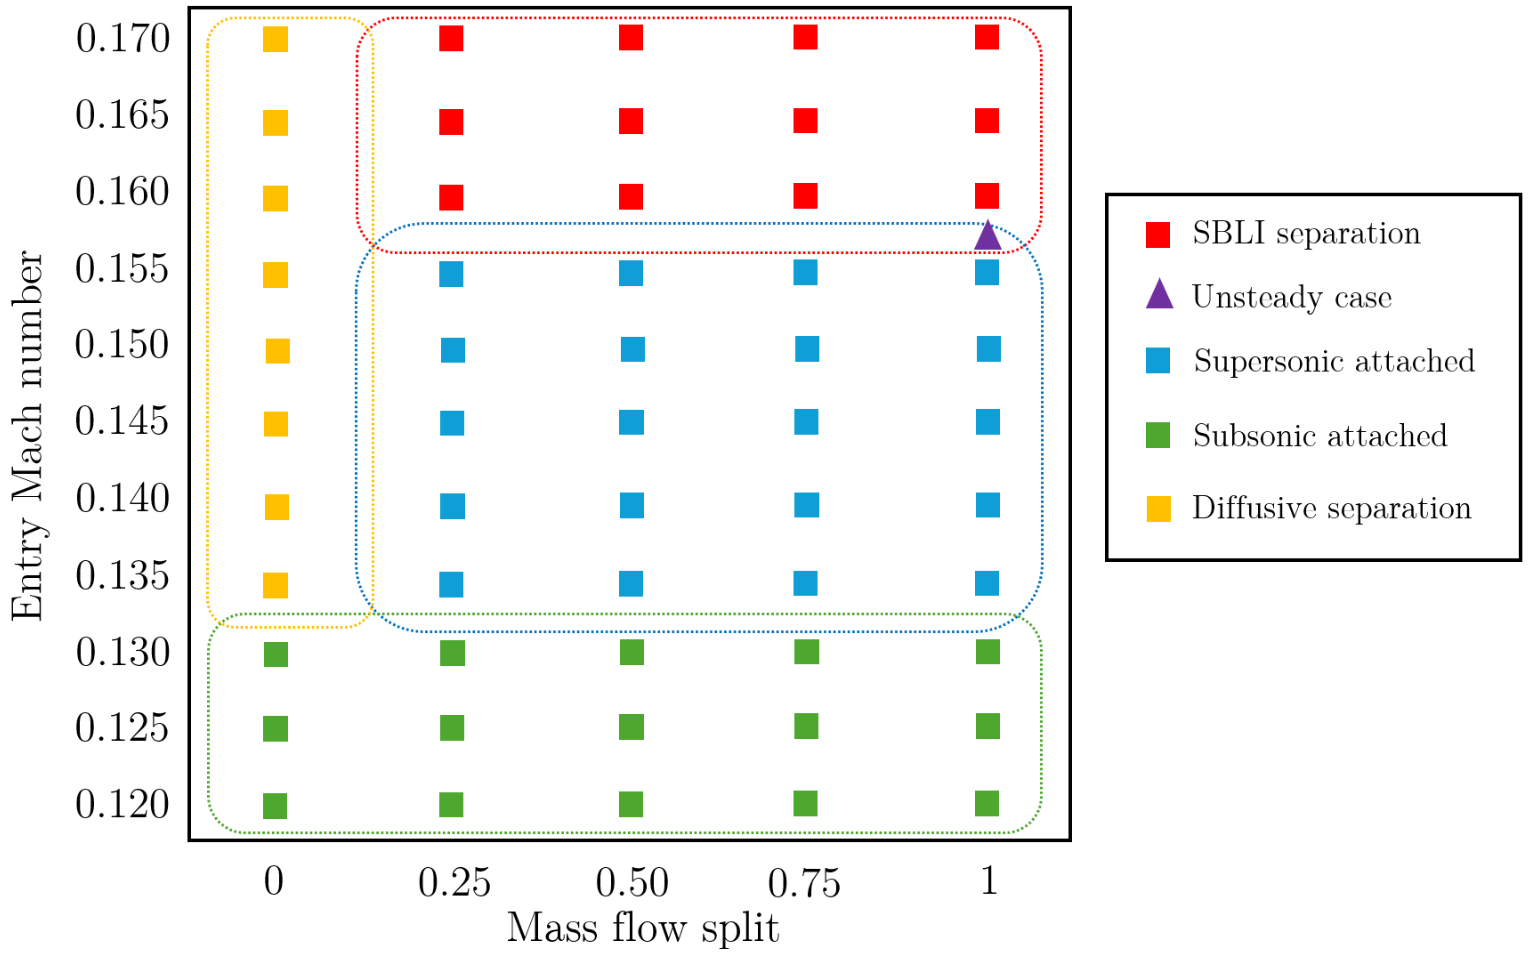
\includegraphics[width=9.2cm,keepaspectratio]{figures/Mach_MFS_space.png}}
    \caption{Flow regime map in $M_{entry}-MFS$ space, adapted from Dickinson.}
  \end{figure}
\end{frame}


\begin{frame}{Why does flow separate at the same Mach number?}
  \begin{columns}[T]
    \column{.5\textwidth}
    \begin{itemize}\setlength\itemsep{.4em}
      \item Flat-plate separation onset at shock Mach number $\approx 1.30$--$1.35$, roughly independent of shape factor $H$
      \item Interaction length $L^*/\delta^* = 70\,(H_i-1)$
      \item Curvature effects on onset: \textbf{disputed} in literature
      \item Separation bubbles can reduce shock drag but raise buffet risk
    \end{itemize}
    \column{.47\textwidth}\centering
    \placeholder{5.6cm}{4.4cm}{Fig.: attached vs.\ separated\\transonic SBLI}
  \end{columns}
\end{frame}


\begin{frame}{Diagnostics and analysis pipeline}
  \begin{columns}[T]
    \column{.4\textwidth}
    \textbf{Measurements}
    \begin{itemize}\setlength\itemsep{.3em}
      \item High-speed shadowgraph, 50\,kHz
      \item Surface static pressures
    \end{itemize}
    \column{.56\textwidth}
    \textbf{Analysis}\vspace{2pt}\\
    \begin{tikzpicture}[node distance=.35cm,
        s/.style={draw=none,fill=mist,rounded corners=3pt,minimum width=5.1cm,minimum height=.62cm,font=\scriptsize,text=navy}]
      \node[s,fill=teal,text=white](a){\bfseries Pixel statistics (mean, SD, kurtosis)};
      \node[s,below=of a](b){Shock tracking: $x_s(t)$, $\sigma_{x_s}$, PDF};
      \node[s,below=of b](c){$x$--$t$ diagrams, Welch PSD, Strouhal number};
      \node[s,below=of c](d){Intermittency $\gamma(x)$, bubble state, dwell times};
      \node[s,below=of d](e){POD / DMD modes};
      \foreach \i/\j in {a/b,b/c,c/d,d/e}{\draw[-{Latex[length=1.5mm]},teal] (\i) -- (\j);}
    \end{tikzpicture}
  \end{columns}
\end{frame}
